\stopallthesefloats
\subsection{Multi-Core Analysis using only UPPAAL}
The authors \cite{conf/wcet/GustavssonELP10} present an approach using UPPAAL
to perform computation of the worst-case execution time for software running
on multi-core processors. While it does not feature cache coherence, it does
support hierarchical (and shared) caches, as well as some sort of instruction
pipelining.

\begin{figure}[hbt!]
\begin{center}
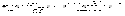
\includegraphics[width=\textwidth]{\chapterdirectory/figure/analysis/gustavsson_prog.pdf}
\end{center}
\caption{Program Automaton (taken from \cite{conf/wcet/GustavssonELP10})}%
\label{fig:formal_analysis:gustavsson_program}
\end{figure}

In \cite{conf/wcet/GustavssonELP10}, programs are represented by their own
automata (See Figure~\ref{fig:formal_analysis:gustavsson_program}), sending
instructions through shared variables by synchronizing with a core on
a dedicated channel. This approach allows programs to feature branching and
non-memory-related instructions, by simply adding numerical variables and
making the automaton more than a simple sequence of states. In
Figure~\ref{fig:formal_analysis:gustavsson_program}, the framed part corresponds
to where the program's instruction graph should be. The \textit{id} variable
targets a particular core on which to execute the instruction, and
\textit{set\_access\_info} populates the global variables characterizing the
instruction: \textit{instr\_address} for the address of the instruction in the
modeled memory, \textit{data\_address} for the address of any data being
accessed, \textit{data\_access} to indicate if this instruction accesses data,
and \textit{write\_data} to differentiate between a read and a write access.
The \textit{Terminating Synchronization} part is here to ensure the task is not
considered completed until it has indeed completed all accesses for its final
instruction (and not just sent the instruction).

Cores are modeled as automata that go through the pipeline required for an
instruction to be completed, which includes accessing the instruction cache as
well as, potentially, the data cache. Interestingly enough, this model does not
use one automaton per stage of the pipeline. Instead the whole core logic is
modeled in a single automaton.


\begin{figure}[hbt!]
\begin{center}
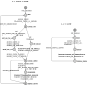
\includegraphics[width=\textwidth]{\chapterdirectory/figure/analysis/gustavsson_caches.pdf}
\end{center}
\caption{Cache Automata (taken from \cite{conf/wcet/GustavssonELP10})}%
\label{fig:formal_analysis:gustavsson_caches}
\end{figure}

Each L1 instruction cache has its own automaton, managing the possibility for
instructions to have already been cached or sending a request for that
instruction to the L2 cache. The L1 data caches are similar (see
Figure~\ref{fig:formal_analysis:gustavsson_caches}), with the added possibility
of writing data to a memory element, which invalidates it from every other L1
data cache.

The automaton for the L2 cache is very straightforward, a simple loop going
over each request, determining whether the data is supposed to be in the L2
cache or not, and delaying the reply accordingly.

\iffalse
An extra automaton is also provided, which acts as a mutex for use in modeling
the programs.
\fi

Unsurprisingly, the hampering factor is scalability when the number of modeled
cores is increased. There appear to have very little in the way of synchronicity
between the cores (such as using a round-robin for L2 cache accesses), which
is likely to be aggravating the issue.
\stopallthesefloats
